% Projective Periodicity Visualization
% Professional redesign with proper spacing and grid layout

\begin{figure}[ht]
\centering
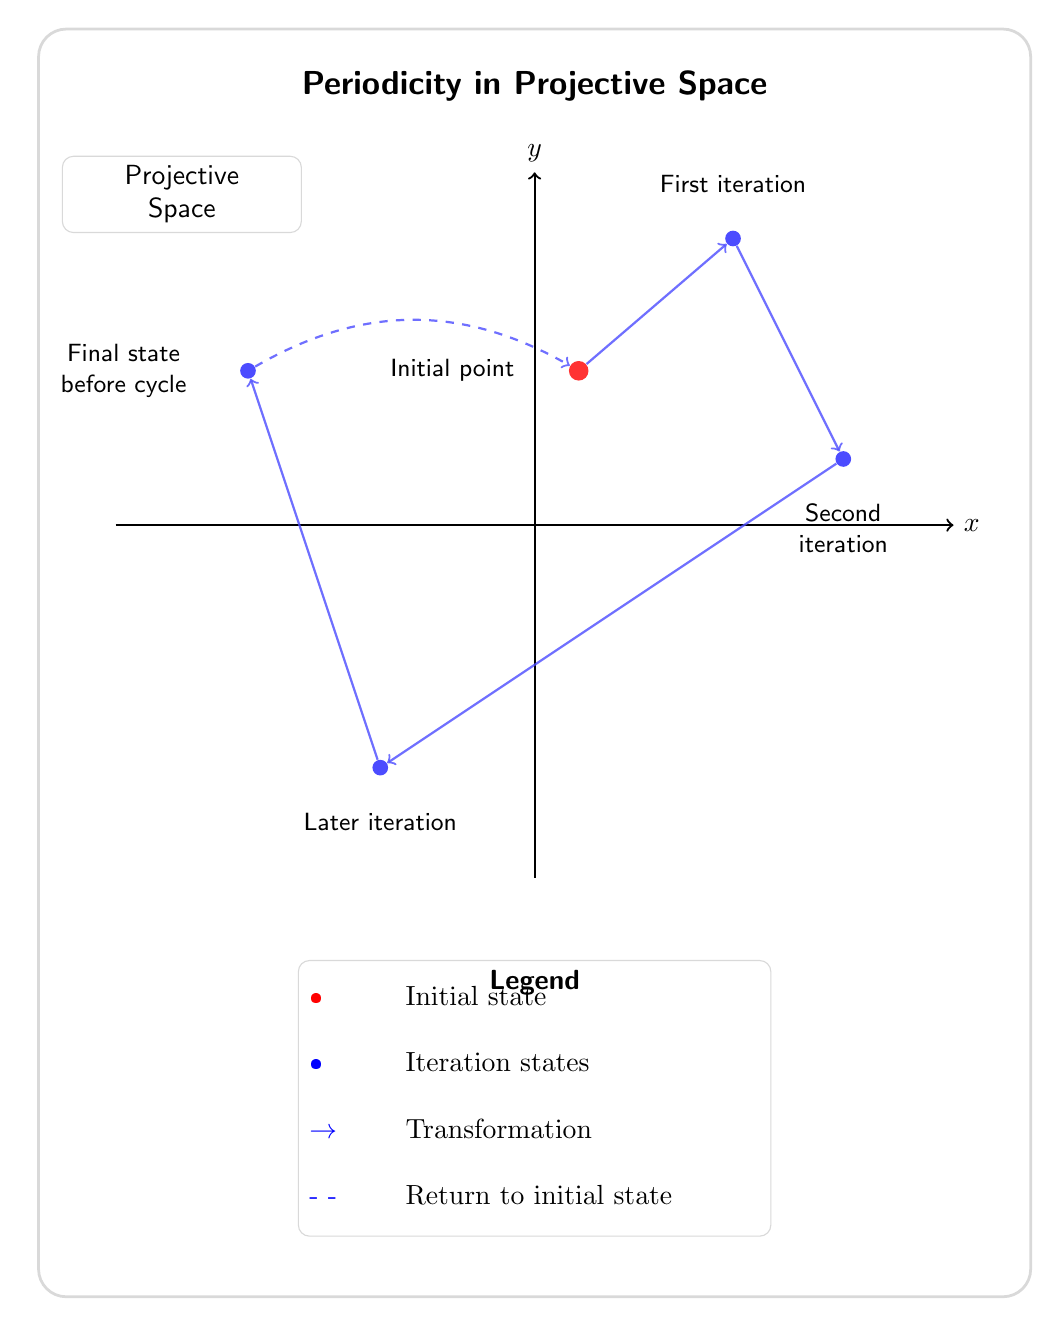
\begin{tikzpicture}[
    scale=1.4,
    point/.style={circle, fill, inner sep=2pt},
    trajectory/.style={->, thick, opacity=0.8},
    label/.style={font=\small\sffamily, align=center, text width=2.2cm}
]
    % Clean background with boundary - Make taller
    \fill[white, rounded corners=10pt, draw=gray!30, line width=1pt] 
        (-4.5,-7) rectangle (4.5,4.5);

    % Title with proper spacing - Move higher
    \node[font=\bfseries\sffamily\large, align=center, anchor=north] 
        at (0,4.2) {Periodicity in Projective Space};
        
    % Main diagram area - centered axes - Spaced further apart
    \draw[->, thick] (-3.8,0) -- (3.8,0) node[right] {$x$};
    \draw[->, thick] (0,-3.2) -- (0,3.2) node[above] {$y$};
    
    % Add proper label for projective space - Move to better position
    \node[fill=white, text opacity=1, fill opacity=0.8, draw=gray!30,
          rounded corners, minimum height=0.8cm, text width=2.8cm, 
          align=center, font=\sffamily] 
          at (-3.2,3) {Projective\\Space};
    
    % Trajectory points - Spread further apart vertically and horizontally
    \node[point, fill=red!80, inner sep=2.5pt] (p0) at (0.4,1.4) {};
    \node[point, fill=blue!70] (p1) at (1.8,2.6) {};
    \node[point, fill=blue!70] (p2) at (2.8,0.6) {};
    \node[point, fill=blue!70] (p3) at (-1.4,-2.2) {};
    \node[point, fill=blue!70] (p4) at (-2.6,1.4) {};
    
    % Connecting arrows - smoother trajectory
    \draw[trajectory, blue!70] (p0) -- (p1);
    \draw[trajectory, blue!70] (p1) -- (p2);
    \draw[trajectory, blue!70] (p2) -- (p3);
    \draw[trajectory, blue!70] (p3) -- (p4);
    \draw[trajectory, blue!70, dashed] (p4) to[bend left=30] (p0);
    
    % Clear labels - Better positioned with controlled width and larger offsets
    \node[label, anchor=east, xshift=-0.25cm] at (p0.west) {Initial point};
    \node[label, anchor=south, yshift=0.35cm] at (p1.north) {First iteration};
    \node[label, anchor=north, yshift=-0.35cm] at (p2.south) {Second iteration};
    \node[label, anchor=north, yshift=-0.35cm] at (p3.south) {Later iteration};
    \node[label, anchor=east, xshift=-0.25cm] at (p4.west) {Final state\\before cycle};
    
    % Legend - More vertical distance from points and larger gaps between items
    \node[draw=gray!30, fill=white, rounded corners, 
          minimum width=6cm, minimum height=3.5cm] (legend) at (0,-5.2) {};
    
    \node[font=\bfseries\sffamily, anchor=north] 
        at (legend.north) {Legend};
    
    \node[anchor=center] at (legend) {
        \begin{tabular}{p{0.8cm}p{4.5cm}}
            \textcolor{red}{\textbullet} & Initial state \\[1.2em]
            \textcolor{blue}{\textbullet} & Iteration states \\[1.2em]
            \textcolor{blue}{$\rightarrow$} & Transformation \\[1.2em]
            \textcolor{blue}{- -} & Return to initial state
        \end{tabular}
    };
    
\end{tikzpicture}
\caption{Visualization of how a periodic cubic irrational creates a closed loop in projective space. The HAPD algorithm detects this pattern by tracking when a point returns to a projectively equivalent position.}
\label{fig:projective_periodicity}
\end{figure} 